\documentclass{scrreprt}
\usepackage{listings}
\usepackage{underscore}
\usepackage[bookmarks=true]{hyperref}
\usepackage[utf8]{inputenc}
\usepackage[english]{babel}
\usepackage{graphicx}
\usepackage[export]{adjustbox}
\usepackage{subcaption}
\hypersetup{
    bookmarks=false,    % show bookmarks bar?
    pdftitle={Machine Learning Report},    % title
    pdfauthor={},                     % author
    pdfsubject={TeX and LaTeX},                        % subject of the document
    pdfkeywords={TeX, LaTeX, graphics, images}, % list of keywords
    colorlinks=true,       % false: boxed links; true: colored links
    linkcolor=blue,       % color of internal links
    citecolor=black,       % color of links to bibliography
    filecolor=black,        % color of file links
    urlcolor=purple,        % color of external links
    linktoc=page            % only page is linked
}%
\def\myversion{1.0 }
\date{}

\usepackage{hyperref}
\begin{document}

\begin{flushright}
    \rule{16cm}{5pt}\vskip1cm
    \begin{bfseries}
        \begin{Huge}{ML Hackathon \\ \begin{large}E-commerce Advertisement Analysis\end{large}\\}\end{Huge}
		\vspace{1.5cm}   
        \today\\
        \vspace{12cm}
        
		\begin{large}
		\begin{center}Crooked Three  \\     
          \vspace{1cm}
         Sriram G.  \hspace{3cm} Ravi Kiran \hspace{3cm} S. Purvaj\\
         (IMT2017018) \hspace{2.25cm}(IMT2017034)\hspace{2cm}(IMT2017039)\\
        \vspace{1.5cm}
		\end{center}
%        \today\\
        \end{large}
    \end{bfseries}
\end{flushright}

\tableofcontents




\chapter{Introduction}

\section{About the problem statement}
In today's scenario e-commerce companies play an integral part in the economy and also there is a lot of analysis required for the companies to asses themselves  an The problem is to predict whether an advertisement on a webpage has been clicked by a user or not based on system data, app/webpage data and advertisement data. This is generally used by large e commerce companies to track their sales and also see which websites are more influential and try to increase their sales by choosing partner websites to advertise customized products for the users. 
\section{References}

\begin{itemize}
\item Analytics Vidhay : WNS wizard 2019 hackathon
\item Medium 
\item Stackoverflow
\end{itemize}



\chapter{Data}
Drive Link for Data :
{\color{blue}{ \\ https://drive.google.com/open?id=1wxn1bqwKrXXeEeYc47kjkuQKauzppp3f}}
\section{Exploration of data}
The data for the problem is across three seperate csv files. One has information about the app, operating system, network used and time of the impression(time at which the data point was recorded) along with the prediction label. Lets call this file/table \textit{impression_info}. Second file has information about the user and device used by the user. Lets call this file/table \textit{user_info}. The third file contains information on the item advertised and the its price. Lets call this file/table \textit{item_info}.

The impression info consists of the data about the impression i.e. the advertisement in the partner website. The system log info consists of the information about the user's interaction with the actual website itself.
Item data consists of the information item that the user has seen when he last logged into the actual website.

\section{Data Analysis}
Firstly, there are no null values across all the three data files. Secondly, the three data files cannot be combined directly as they are of different sizes. The file which contains the prediction labels is governs how much training data is available which in our case is the \textit{impression_info} file. We must join this file in an appropriate way so that we can extract suitable features from the whole dataset. Now, we have the complete dataset with about *** data points.

Another important observaion about the given data is that it is highly biased. Only $5\%$ of the given data is positive while the remaining $95\%$ data is negative.

Some of the plots that we used to understand the data better have been shown in the following page:

\begin{figure}[!h]
\centering
\begin{subfigure}{.5\textwidth}
  \centering
  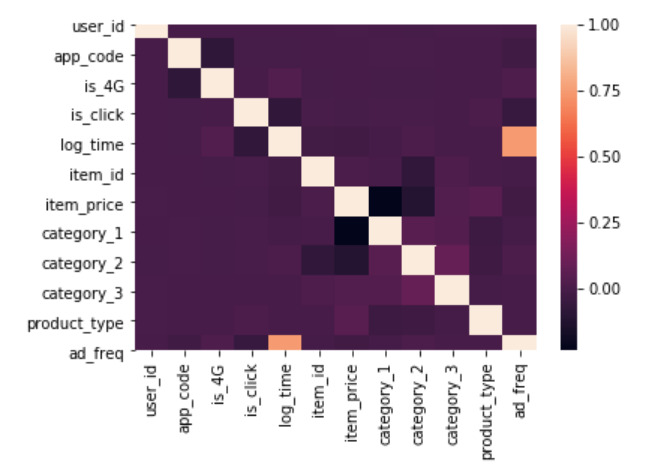
\includegraphics[scale=0.30]{1}
  \caption{Correlation Plot}
\end{subfigure}%
\begin{subfigure}{.5\textwidth}
  \centering
  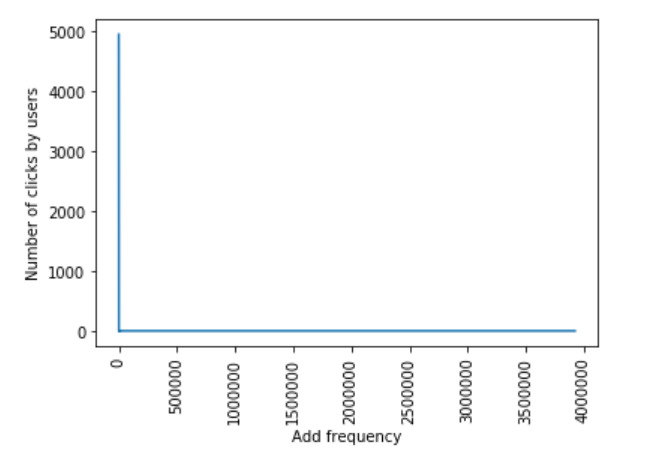
\includegraphics[scale=0.30]{2}
  \caption{Add frequency vs Number of clicks}
\end{subfigure}%

\begin{subfigure}{.5\textwidth}
  \centering
  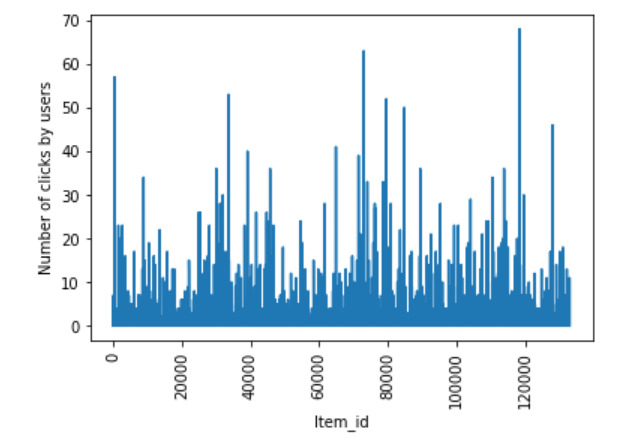
\includegraphics[scale=0.30]{3}
  \caption{Item id vs Number of clicks}
\end{subfigure}%
\begin{subfigure}{.5\textwidth}
  \centering
  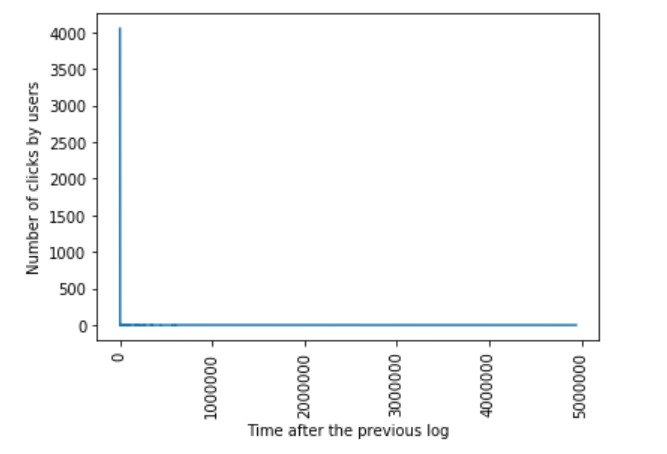
\includegraphics[scale=0.30]{4}
  \caption{Item id vs Number of clicks}
\end{subfigure}

\caption{ Data Analysis}
\end{figure}

\section{Data Pre-processing and Feature Engineering}
The impression ids for a specific user are only after he logs into the system atleast ones. Therefore each impression that a user encounters between two successive logs is related only to the item that the user has seen in the previous log. We use this technique to join the data files in a sensible manner.
\subsection{Time duration between log time and impression time:}
This feature is calculated as the time difference between the most recent log time(the most recent time instant at which the user was logged onto the app/website) and the impression time(the time instant at which the advertisement appears to the user) in seconds. \\
After looking at the data we found out that the data can be understood as below: \\
($T_1$) \textbf{log entry of user 1} --------------------------------------------------------------------\\
($T_2$)		\qquad	++++++++++++++++++++ \qquad impid_1 user_1 \\
($T_3$)		\qquad	++++++++++++++++++++ \qquad impid_2 user_1 \\
($T_4$)		\qquad	++++++++++++++++++++ \qquad impid_3 user_1 \\
($T_5$)		\qquad	++++++++++++++++++++ \qquad impid_4 user_1 \\
($T_6$) \textbf{log entry of user 2} --------------------------------------------------------------------\\
($T_7$)		\qquad	++++++++++++++++++++ \qquad impid_5 user_2 \\
($T_8$)		\qquad	++++++++++++++++++++ \qquad impid_6 user_2 \\
($T_9$)		\qquad	++++++++++++++++++++ \qquad impid_7 user_1 \\
($T_{10}$)	\qquad  ++++++++++++++++++++ \qquad impid_8 user_1 \\
($T_{11}$) \textbf{log entry of user 1} ------------------------------------------------------------------\\
($T_{12}$)	\qquad  ++++++++++++++++++++ \qquad impid_9 user_1 \\
($T_{13}$)	\qquad	++++++++++++++++++++ \qquad impid_10 user_1 \\
($T_{14}$)	\qquad	++++++++++++++++++++ \qquad impid_11 user_2 \\


In the above example the user 1 logs at an instant time_1 and then there are many impression ids. Now each impression id for the user_1 between T(1) and T(10) will only be aboutthe item that he searched for, when he entered for the first time. We create a new column which contains the difference between the time at which the user logs into the system and the time at which the user encounters the impression id.

$(T_i) - (T_j)$ where $i>j$ and i $\epsilon \{1,6,11\}$ and j $\epsilon \{2,3,4,5,7,8,9,10,12,23,14\}$ depending on the user id.
					
					
\subsection{Item_id from recent log}
The second feature that was extracted was the details of the item that the user checked in the last log. This might useful for the situation when the user's probability of buying a specific item is based on his/her's previous history of buying products.
Hence the user_id is not removed from the training data and is also used as a feature.

\subsection{Add frequency}
The third feature that was extracted was the details of the frequency at which the user was seeing the ads of that particular website.Now we finally end up 11 features for training the models. 

\subsection{Pre processing}
Initial step was to normalize the data and to convert the categorical attributes into integers.
Then we used PCA to reduce the dimensionality of the data.We tried using multiple values for components of the pca reducability. 
We have seen that the data is higly biased. Therefore we have used some techniques to generalize the model.
We split the negative data(is_click=0) into 20 groups and trained these data groups along with the positive data in different models and used voting classifier for training. 

For testing and prediction, we considered the outputs of the various models trained as described above. We considered the class that the majority of the models predicted as our prediction.
\chapter{Model Selection and Building} 


\section{Model-1: Logistic Regression}
Logistic regression is one of the simple binary classifier that is based on a log loss .
W is the weight matrix and x is the data matrix. B is the bias.
\begin{center}
	Hypothesis : Z = WX+ b
	\\
	$h(\theta(x))  = sigmoid(Z)$ 
	\\
\end{center}
	where sigmoid is 
\begin{center} 
		$sigmoid(x) = \frac{1}{1+e^{-x}}$
\end{center}

\subsubsection{Theory}

\subsubsection{results:}
	Considered data of size 22000(estimated) \\
	Accuracy** : 69.49\%

\section{Model-2: XGB Classifier}
	

\subsubsection{Theory}

\subsubsection{Results:}
	Considered data of size 22000(estimated) \\
	Accuracy** : 98.49\%


\section{Model-3: Random Forest Classifier}

\subsubsection{Theory}
Random Forest uses the idea of Decision Trees. It takes a random subset of features and builds the decision tree and then uses it for prediction.

\subsubsection{Results:}
	Considered data of size 22000(estimated) \\
	Accuracy** : 98.21\%
%	Confusion Matrix

\section{Model-4: Voting Classifier}

\subsubsection{Theory}
It is an ensemble of the above models and then predicts based on importance.

\subsubsection{Results:}
	Considered data of size 22000(estimated) \\
	Accuracy** : 98.48 \%


\chapter{Observations and Results}

\begin{center}
 \begin{tabular}{||c | c | c | c||} 
 \hline
 Model & PCA-6 & PCA-7 & without PCA \\ [0.5ex] 
 \hline\hline
 Logistic Regression & 73.47\% & 73.47\% & 69.49\%\\ 
 \hline
 Random Forest Classifier & 97.45\% & 97.07\% & 98.21\%\\
 \hline
 XGB Classifier & 97.31\% & 97.2\% & 98.49\%\\
 \hline
 Voting Classifier & 97.31\% & 97.17\% & 98.48\% \\
 \hline
\end{tabular}
\end{center}
**Accuracy mentioned in the above is an average over a set of 20 different variables.


\end{document}
